% - incremental
\section{Incremental}
\begin{frame}{Concept}
    \begin{minipage}{0.5\textwidth}
        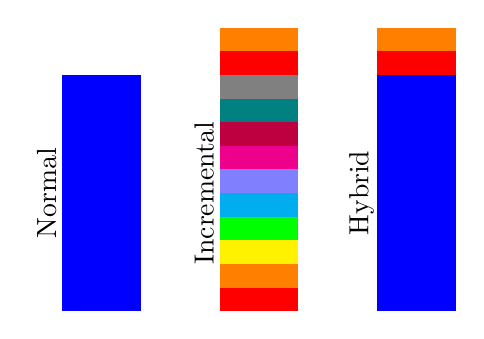
\begin{tikzpicture}

            % First pillar (blue)
            \fill[blue] (0,0) rectangle (1,3);
            \node[rotate=90] at (-0.2, 1.5) {Normal};

            % Second pillar (split into 10 different colors)
            \fill[red] (2,0) rectangle (3,0.3);
            \fill[orange] (2,0.3) rectangle (3,0.6);
            \fill[yellow] (2,0.6) rectangle (3,0.9);
            \fill[green] (2,0.9) rectangle (3,1.2);
            \fill[cyan] (2,1.2) rectangle (3,1.5);
            \fill[blue!50] (2,1.5) rectangle (3,1.8);
            \fill[magenta] (2,1.8) rectangle (3,2.1);
            \fill[purple] (2,2.1) rectangle (3,2.4);
            \fill[teal] (2,2.4) rectangle (3,2.7);
            \fill[gray] (2,2.7) rectangle (3,3);
            \fill[red] (2,3) rectangle (3,3.3);
            \fill[orange] (2,3.3) rectangle (3,3.6);
            \node[rotate=90] at (1.8, 1.5) {Incremental};

            % Third pillar (blue with colorful segments on top)
            \fill[blue] (4,0) rectangle (5,3);
            \fill[red] (4,3) rectangle (5,3.3);
            \fill[orange] (4,3.3) rectangle (5,3.6);
            \node[rotate=90] at (3.8, 1.5) {Hybrid};

        \end{tikzpicture}
    \end{minipage}%
    \begin{minipage}{0.5\textwidth}
        \begin{itemize}
            \item solving for every timestep
            \item worse in comparison with good estimate
            \item hybrid to get both good time and adaptability
        \end{itemize}
    \end{minipage}
\end{frame}

\begin{frame}{Split}
    \begin{minipage}{0.5\textwidth}
        \begin{tcolorbox}[colframe=black, colback=white, sharp corners=southwest, boxrule=0.5mm]
            \texttt{base}
            \begin{itemize}
                \item input conversion
                \item malfunction conversion
                \item pathfinding
            \end{itemize}
        \end{tcolorbox}
    \end{minipage}%
    \begin{minipage}{0.5\textwidth}
        \begin{tcolorbox}[colframe=black, colback=white, sharp corners=northwest, boxrule=0.5mm]
            \texttt{step}
            \begin{itemize}
                \item pathfinding (stepwise)
            \end{itemize}
        \end{tcolorbox}
        \vspace{0.5cm} % Add space between step and check
        \begin{tcolorbox}[colframe=black, colback=white, sharp corners=southeast, boxrule=0.5mm]
            \texttt{check}
            \begin{itemize}
                \item goal condition
            \end{itemize}
        \end{tcolorbox}
    \end{minipage}
\end{frame}